% ============================================================================
% IEEE Conference Paper — Digital Inclusion & Circular Economy in India
% Authors: Yash Chauhan, Shreya Srivastava
% Date: February 2026
% Format: IEEE Conference (Two-Column)
% ============================================================================

\PassOptionsToPackage{hyphens}{url}

\documentclass[conference]{IEEEtran}

% ── Packages ────────────────────────────────────────────────────────────────
\usepackage{cite}
\usepackage{amsmath,amssymb,amsfonts}
\usepackage{newtxtext,newtxmath}
\usepackage{graphicx}
\usepackage{textcomp}
\usepackage{xcolor}
\usepackage{balance}
\usepackage{booktabs}       % Professional tables
\usepackage{multirow}       % Multi-row table cells
\usepackage{array}          % Extended column formatting
% \usepackage{caption}        % (REMOVED) Interferes with IEEEtran native formatting
% \usepackage{subcaption}     % (REMOVED) Interferes with IEEEtran native formatting
\usepackage[caption=false, font=footnotesize]{subfig} % IEEE recommended for subfigures
\usepackage{hyperref}

% ── Custom Commands ─────────────────────────────────────────────────────────
\providecommand{\textrupee}{Rs.}  % Indian Rupee symbol (fallback)

\hypersetup{
    colorlinks=true,
    linkcolor=black,
    citecolor=black,
    urlcolor=black
}
\Urlmuskip=0mu plus 1mu\relax

\def\BibTeX{{\rm B\kern-.05em{I}\kern-.025em b\kern-.08em
    T\kern-.1667em\lower.7ex\hbox{E}\kern-.125emX}}

% ============================================================================
\begin{document}

% ── Title ───────────────────────────────────────────────────────────────────
\title{Digital Inclusion and Circular Economy Behavior in\\Indian States: A Digital Circularity Index and\\Explainable XGBoost Analysis}

% ── Authors ─────────────────────────────────────────────────────────────────
\author{
\IEEEauthorblockN{Suresh Kumar Chelliah}
\IEEEauthorblockA{
\textit{Dept. of Computational Intelligence} \\
\textit{SRM Institute of Science \& Technology} \\
Kattankulathur, Tamil Nadu, India \\
sureshkc@srmist.edu.in}
\and
\IEEEauthorblockN{Shreya Srivastava}
\IEEEauthorblockA{\textit{Dept. of Computational Intelligence} \\
\textit{SRM Institute of Science \& Technology} \\
Kattankulathur, Tamil Nadu, India \\
ss1371@srmist.edu.in}
\and
\IEEEauthorblockN{Yash Chauhan}
\IEEEauthorblockA{\textit{Dept. of Computational Intelligence} \\
\textit{SRM Institute of Science \& Technology} \\
Kattankulathur, Tamil Nadu, India \\
yc0810@srmist.edu.in}
}

\maketitle

% =======s=====================================================================
% ABSTRACT
% ============================================================================
\begin{abstract}
India is simultaneously expanding digital infrastructure and pursuing circular economy goals, yet the relationship between these two agendas remains underexplored at the state level. This study integrates seven official government data sources to construct a Digital Circularity Index (DCI) for 16 Indian states. The analysis combines OLS regression, robustness testing, mediation analysis, threshold analysis, leak-free nested cross-validation, SHAP-based explainability, and K-Means clustering. Across methods, states with stronger digital access consistently show better circular economy outcomes. The association remains significant under non-parametric and permutation-based checks, while tele-density emerges as a stronger driver than digital payments. The results also reveal a substantial gap between digitally advanced and lagging states. These findings suggest that digital inclusion and sustainability policy should be treated as interconnected rather than separate agendas.
\end{abstract}

\begin{IEEEkeywords}
Circular economy, digital circularity index (DCI), digital inclusion, extreme gradient boosting (XGBoost), Shapley additive explanations (SHAP)
\end{IEEEkeywords}

% ============================================================================
% I. INTRODUCTION
% ============================================================================
\section{Introduction}

Since 2015, Digital India has expanded broadband, mobile connectivity, and the Unified Payments Interface (UPI) across a country of 1.4 billion people. Monthly UPI transactions now exceed 14 billion \cite{npci2025}, and national tele-density is above 85\% \cite{trai2024}. At the same time, India generates roughly 62 million tonnes of waste annually and ranks among the world's top three e-waste producers \cite{cpcb2023}. NITI Aayog's circular-economy (CE) strategy now spans 11 priority sectors \cite{nitiCE2021}.

Yet the relationship between these agendas remains underexplored. Digital India research focuses mainly on growth, employment, and financial inclusion \cite{meity2023}, while CE research stays centered on waste-management technology and EPR policy \cite{geissdoerfer2017}. Very little state-level work asks whether stronger digital access is associated with better environmental performance.

\subsection{What This Paper Does}

This paper addresses that gap by constructing a Digital Circularity Index (DCI) from seven official data sources covering 16 Indian states. The analysis combines OLS, non-parametric tests, bootstrap resampling, seven LOO-CV models, nested-CV XGBoost with SHAP, and K-Means clustering. The main contributions are a state-level index linking digital access and CE behavior, cross-method validation of the relationship, and state-specific interpretation through clustering and explainability.

\subsection{Research Questions and Hypotheses}

The central question is straightforward: does digital inclusion predict circular economy performance across Indian states? We formalised this into three testable hypotheses:

\begin{itemize}
    \item \textbf{H1:} States with higher Digital Access Scores will also have higher CE Behavior Scores.
    \item \textbf{H2:} UPI adoption mediates this relationship---i.e., digital payments are the channel through which digital access affects CE behavior.
    \item \textbf{H3:} There is a tele-density threshold beyond which CE behavior improves sharply.
\end{itemize}

% II. LITERATURE SURVEY
% ============================================================================
\section{Literature Survey}

\subsection{Digital Inclusion in India}

Between 2015 and 2024, India pushed tele-density beyond 85\% nationally, while some urban pockets crossed 130\% \cite{trai2024}. Since 2016, UPI has grown into the world's largest real-time digital payments system \cite{npci2025}. But large regional disparities remain: Bihar's tele-density is around 55.80, while Kerala exceeds 120\%. Most research in this area focuses on growth, access expansion, and financial inclusion \cite{meity2023}, leaving the link between digital connectivity and sustainability outcomes relatively underexplored.

\subsection{Circular Economy in India}

The circular economy entered the policy mainstream through the Ellen MacArthur Foundation and was later distinguished more clearly from the broader idea of sustainability by Geissdoerfer \textit{et al.} \cite{emf2013,geissdoerfer2017}. In India, NITI Aayog translated that agenda into an 11-sector strategy \cite{nitiCE2021}, but implementation remains uneven. India generates roughly 1.71 million tonnes of e-waste annually, only part of which enters formal recycling channels \cite{cpcb2023}, and state SDG scores still range from 57 to 79 \cite{nitiSDG2024}.

\subsection{Where Digital and CE Research Miss Each Other}

Avgerou and Heeks argue that ICTs reshape development through multiple channels, including governance, markets, information flow, and institutional functioning \cite{avgerou2010,heeks2017}. If that view holds, digital access should affect CE behavior through several mechanisms rather than one isolated pathway. Even so, state-level evidence connecting Digital India with circular-economy outcomes remains limited. This study addresses that gap.

% ============================================================================
% III. METHODOLOGY
% ============================================================================
\section{Methodology}

\subsection{Research Design}

This study uses a \textbf{cross-sectional} design covering 16 Indian states with complete observations across all seven government sources. We apply an \textbf{inner-join strategy}, favoring consistency and traceability over a larger sample.

\subsection{Data Sources}

\begin{table}[!t]
\centering
\caption{Data Sources and Variables}
\label{tab:data_sources}
\renewcommand{\arraystretch}{1.15}
\begin{tabular}{@{}p{2.2cm}p{2.8cm}p{1.2cm}@{}}
\toprule
\textbf{Source} & \textbf{Variable} & \textbf{Year} \\
\midrule
TRAI \cite{trai2024} & Tele-density (\%) & 2024 \\
RBI \cite{rbi2025} & Per Capita NSDP (INR) & 2023--24 \\
NITI Aayog \cite{nitiSDG2024} & SDG Index Score & 2023--24 \\
NPCI/\newline Dataful \cite{npci2025, dataful2026} & UPI Per Capita Txns & 2024--25 \\
CPCB \cite{cpcb2023} & E-Waste Processed (T) & 2021--22 \\
Census \cite{census2011} & Literacy Rate (\%) & 2011 \\
Census \cite{census2011} & Urban Population (\%) & 2011 \\
\bottomrule
\end{tabular}
\end{table}

After merging the source files, the final dataset contains \textbf{16 states} $\times$ \textbf{15 variables} (9 raw and 6 derived).

\subsection{Composite Index Construction}

\subsubsection{Min-Max Normalization}

Each raw variable $x_i$ is rescaled to a $[0, 100]$ range:

\begin{equation}
    \hat{x}_i = \frac{x_i - x_{\min}}{x_{\max} - x_{\min}} \times 100
\end{equation}

\subsubsection{Digital Access Score (DAS)}

\begin{equation}
    DAS = 0.40 \cdot \hat{T}_d + 0.30 \cdot \hat{U}_{pc} + 0.30 \cdot \hat{N}_{pc}
\end{equation}

\noindent where $\hat{T}_d$ denotes normalized tele-density, $\hat{U}_{pc}$ denotes normalized UPI transactions per capita, and $\hat{N}_{pc}$ denotes normalized per capita NSDP. Tele-density receives the largest weight because it captures underlying communications infrastructure.

\subsubsection{CE Behavior Score (CEBS)}

\begin{equation}
    CEBS = 0.35 \cdot \hat{E}_{pc} + 0.40 \cdot S_{sdg} + 0.25 \cdot \hat{N}_{pc}
\end{equation}

\noindent where $\hat{E}_{pc}$ is normalized e-waste processed per capita, $S_{sdg}$ is the SDG Index Score, and $\hat{N}_{pc}$ is normalized per capita NSDP.

\subsubsection{Digital Circularity Index (DCI)}

\begin{equation}
    DCI = \frac{DAS \times CEBS}{100}
\end{equation}

This multiplicative form requires strength on both dimensions.

\subsection{Statistical Analysis Methods}

H1 is evaluated using an OLS regression of CEBS on DAS:

\begin{equation}
    CEBS_i = \beta_0 + \beta_1 \cdot DAS_i + \varepsilon_i
\end{equation}

\noindent Diagnostics include Breusch-Pagan, Durbin-Watson, and Cook's distance. H2 is tested with the Baron \& Kenny \cite{baron1986} framework and the Sobel test, while H3 uses piecewise regression with grid-searched threshold estimation.

\subsection{Machine Learning Methods}

\subsubsection{Leave-One-Out Cross-Validation (LOO-CV)}

With only $n = 16$ observations, we use LOO-CV:

\begin{equation}
    R^2_{LOO} = 1 - \frac{\sum_{i=1}^{n} (y_i - \hat{y}_{-i})^2}{\sum_{i=1}^{n} (y_i - \bar{y})^2}
\end{equation}

Seven models are compared under this framework.

\subsubsection{Nested LOO-CV with GridSearch}

To avoid hyperparameter leakage, we also implement nested cross-validation with an outer LOO loop for evaluation and an inner 4-fold loop for tuning.

\subsubsection{SHAP Explainability}

Model explainability is handled using SHAP \cite{lundberg2017}:

\begin{equation}
    f(x) = \phi_0 + \sum_{j=1}^{p} \phi_j(x)
\end{equation}

\noindent where $\phi_0$ is the baseline prediction and $\phi_j(x)$ is the contribution of feature $j$ for instance $x$.

\subsubsection{K-Means Clustering}

Finally, K-Means clustering is used to identify state groupings, with the number of clusters selected by silhouette score.

% ============================================================================
% IV. RESULTS
% ============================================================================
\section{Results}

\subsection{Descriptive Statistics}

Table~\ref{tab:descriptive} summarizes DAS, CEBS, and DCI across the 16 states. Bihar records the lowest value on all three indices, while Haryana posts the highest DCI at 72.97 and Karnataka the highest DAS at 94.40.

\begin{table}[!t]
\centering
\caption{Descriptive Statistics of Composite Indices ($n = 16$)}
\label{tab:descriptive}
\renewcommand{\arraystretch}{1.15}
\begin{tabular}{@{}lccc@{}}
\toprule
\textbf{Statistic} & \textbf{DAS} & \textbf{CEBS} & \textbf{DCI} \\
\midrule
Mean        & 64.95 & 46.98 & 32.52 \\
Std. Dev.   & 19.69 & 13.90 & 17.40 \\
Min         & 30.27 & 27.23 & 8.24  \\
Max         & 94.40 & 87.30 & 72.97 \\
Median      & 67.02 & 47.78 & 32.42 \\
\bottomrule
\end{tabular}
\end{table}

Figs.~\ref{fig:dci_ranking} and \ref{fig:heatmap} show the spread clearly. SDG Index, Per Capita NSDP, and Tele-density display the strongest associations with CE Behavior Score.

\begin{figure}[!t]
    \centering
    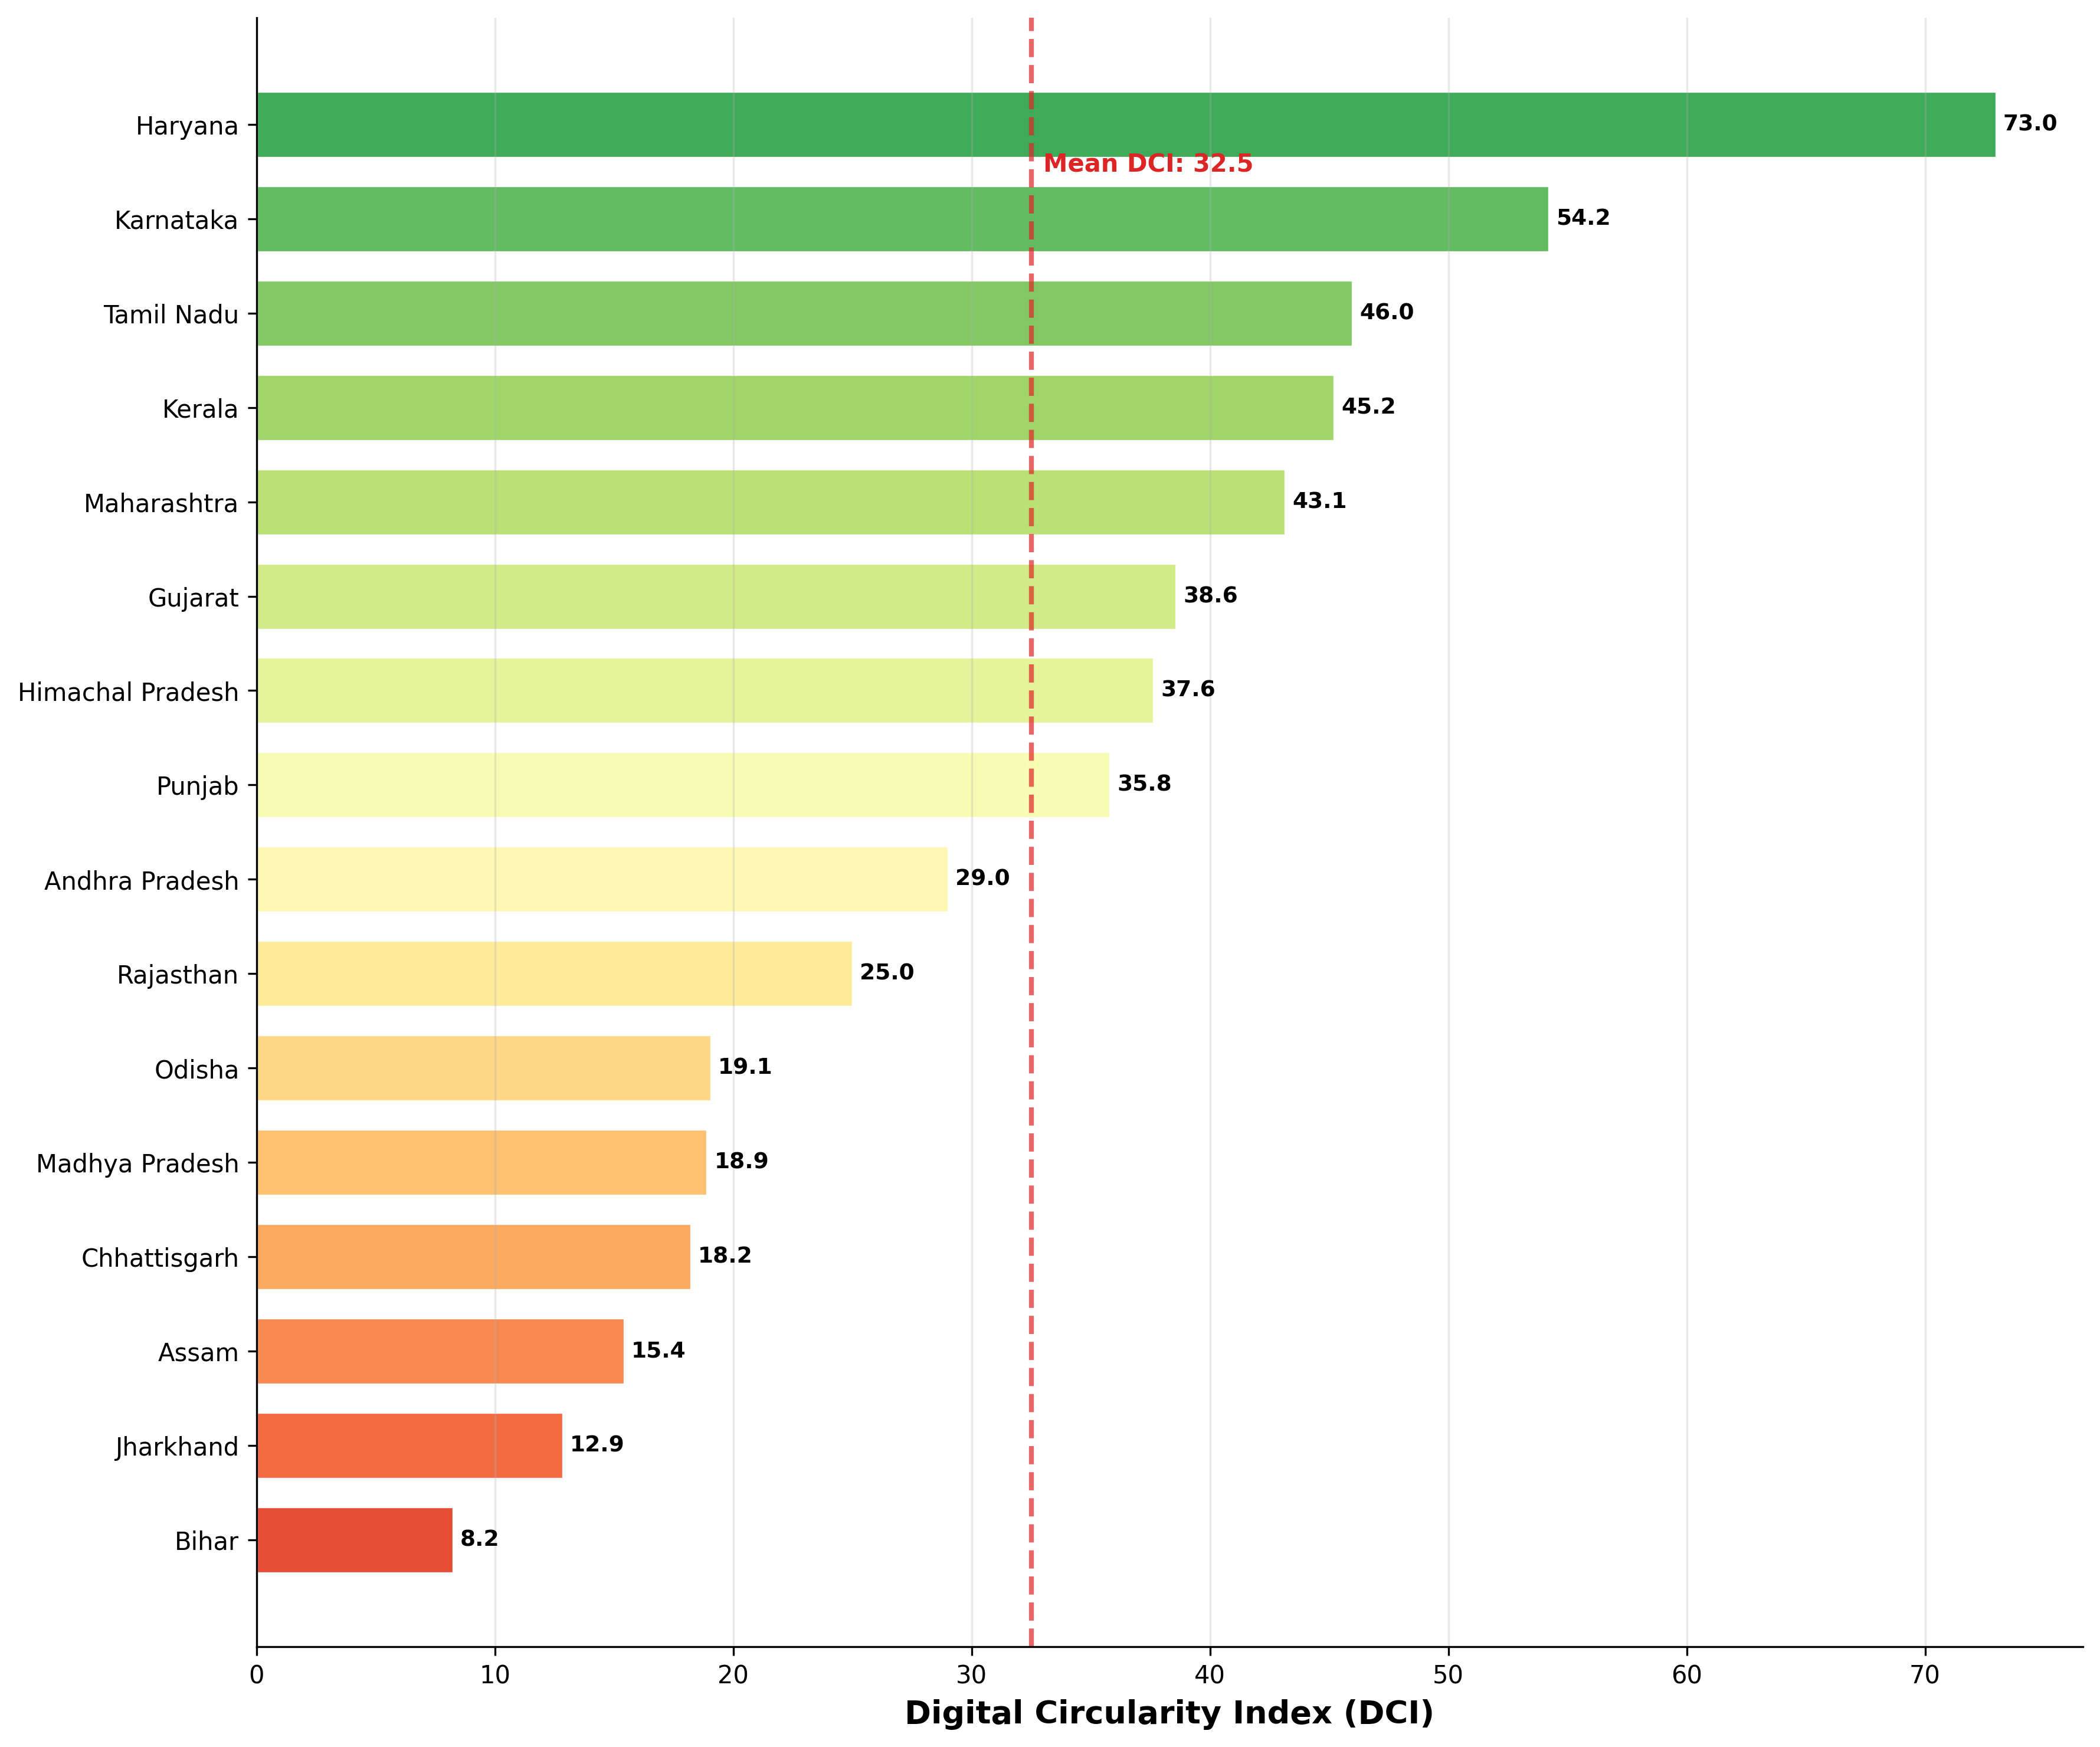
\includegraphics[width=\columnwidth]{figures/fig3_dci_ranking.jpg}
    \caption{Digital Circularity Index (DCI) ranking across 16 Indian states. Haryana leads (72.97), Bihar lags (8.24).}
    \label{fig:dci_ranking}
\end{figure}

\begin{figure}[!t]
    \centering
    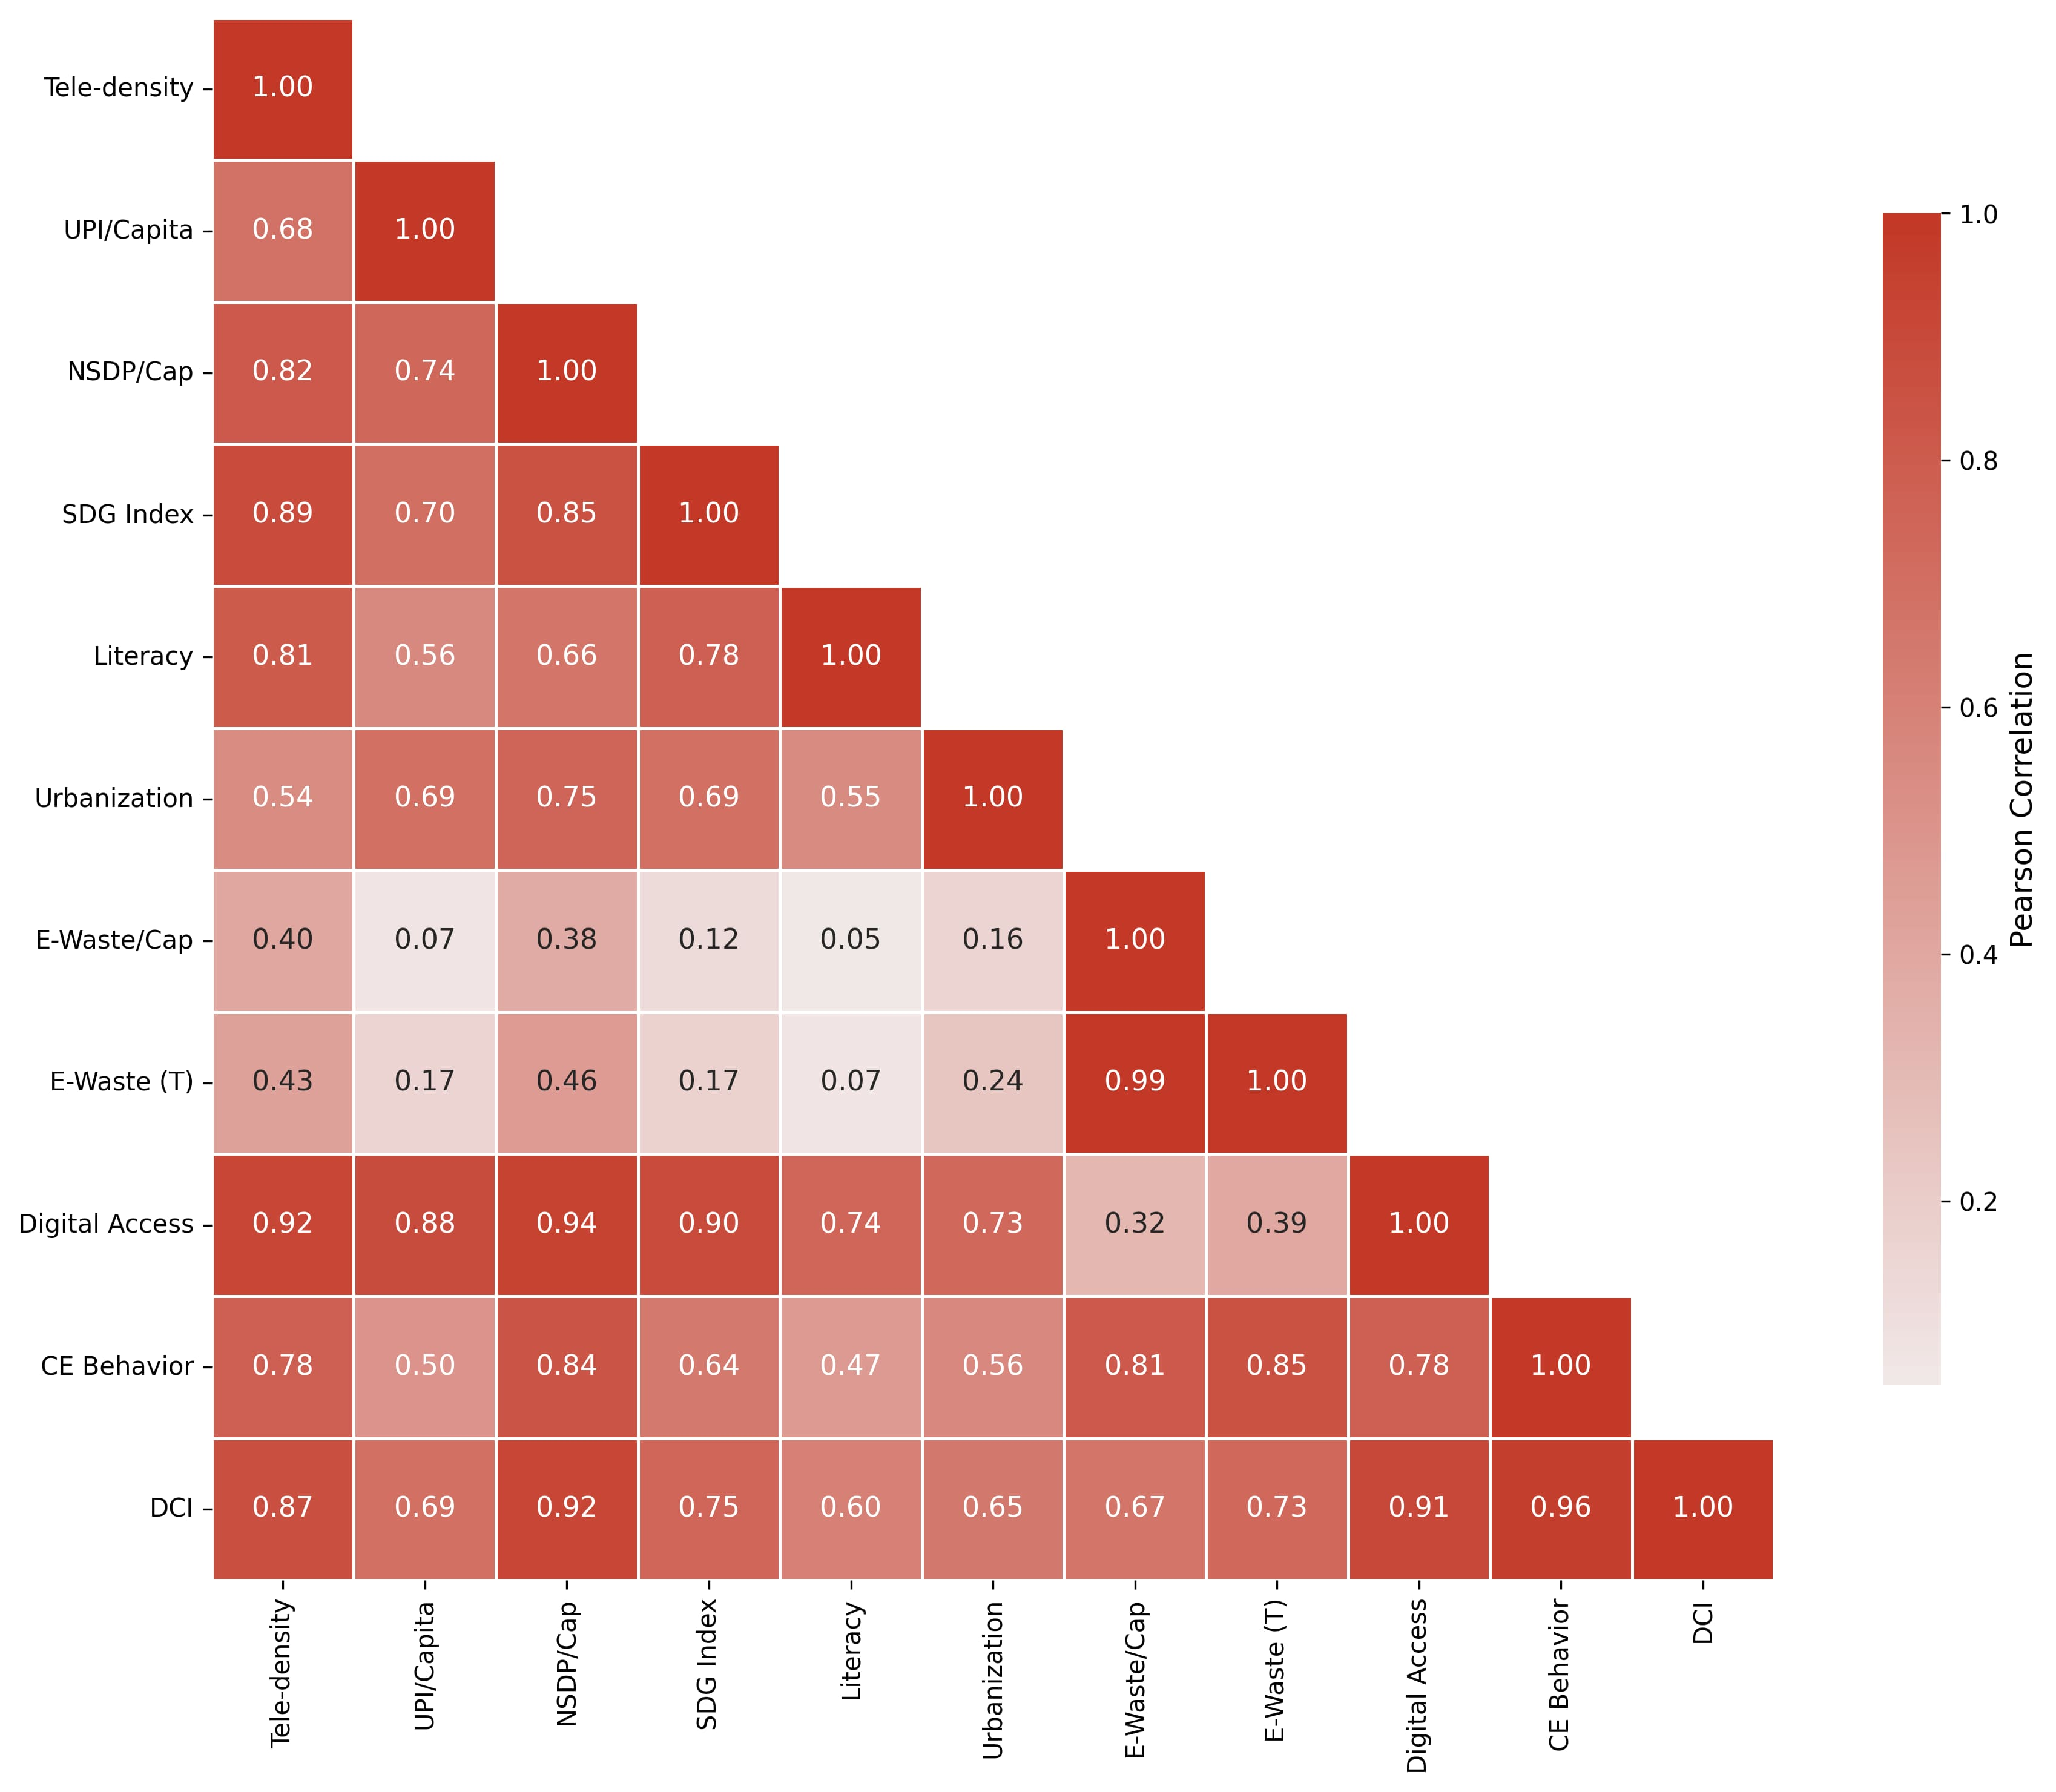
\includegraphics[width=\columnwidth]{figures/fig1_correlation_heatmap.jpg}
    \caption{Correlation heatmap of all numeric variables. Darker colors indicate stronger correlations.}
    \label{fig:heatmap}
\end{figure}

\subsection{Primary Regression Analysis (H1)}

The fitted OLS model is:

\begin{equation}
    CEBS = 11.158 + 0.551 \cdot DAS
    \label{eq:ols_result}
\end{equation}

A one-point increase in DAS is associated with roughly a 0.55-point increase in CEBS. The model explains 61\% of the variance, and the coefficient remains significant at $p < 0.001$, supporting H1.

\begin{table}[!t]
\centering
\caption{OLS Regression Results --- Primary Model}
\label{tab:ols}
\renewcommand{\arraystretch}{1.15}
\begin{tabular}{@{}lc@{}}
\toprule
\textbf{Metric} & \textbf{Value} \\
\midrule
$R^2$               & 0.610 \\
Adjusted $R^2$      & 0.583 \\
$\beta_1$ (slope)   & 0.551 \\
SE($\beta_1$)       & 0.118 \\
$t$-statistic       & 4.684 \\
$p$-value            & 0.000352 \\
$F$-statistic        & 21.94 \\
95\% CI for $\beta_1$ & [0.299, 0.804] \\
Pearson $r$          & \textbf{0.781} \\
\bottomrule
\end{tabular}
\end{table}

A five-control specification raises $R^2$ to 0.763, but it also introduces clear multicollinearity: the VIF reaches 10.57 for DAS and 9.47 for NSDP. Because NSDP is built into both composite scores, the bivariate model in Eq.~\ref{eq:ols_result} remains the cleaner test of H1.

\begin{figure}[!t]
    \centering
    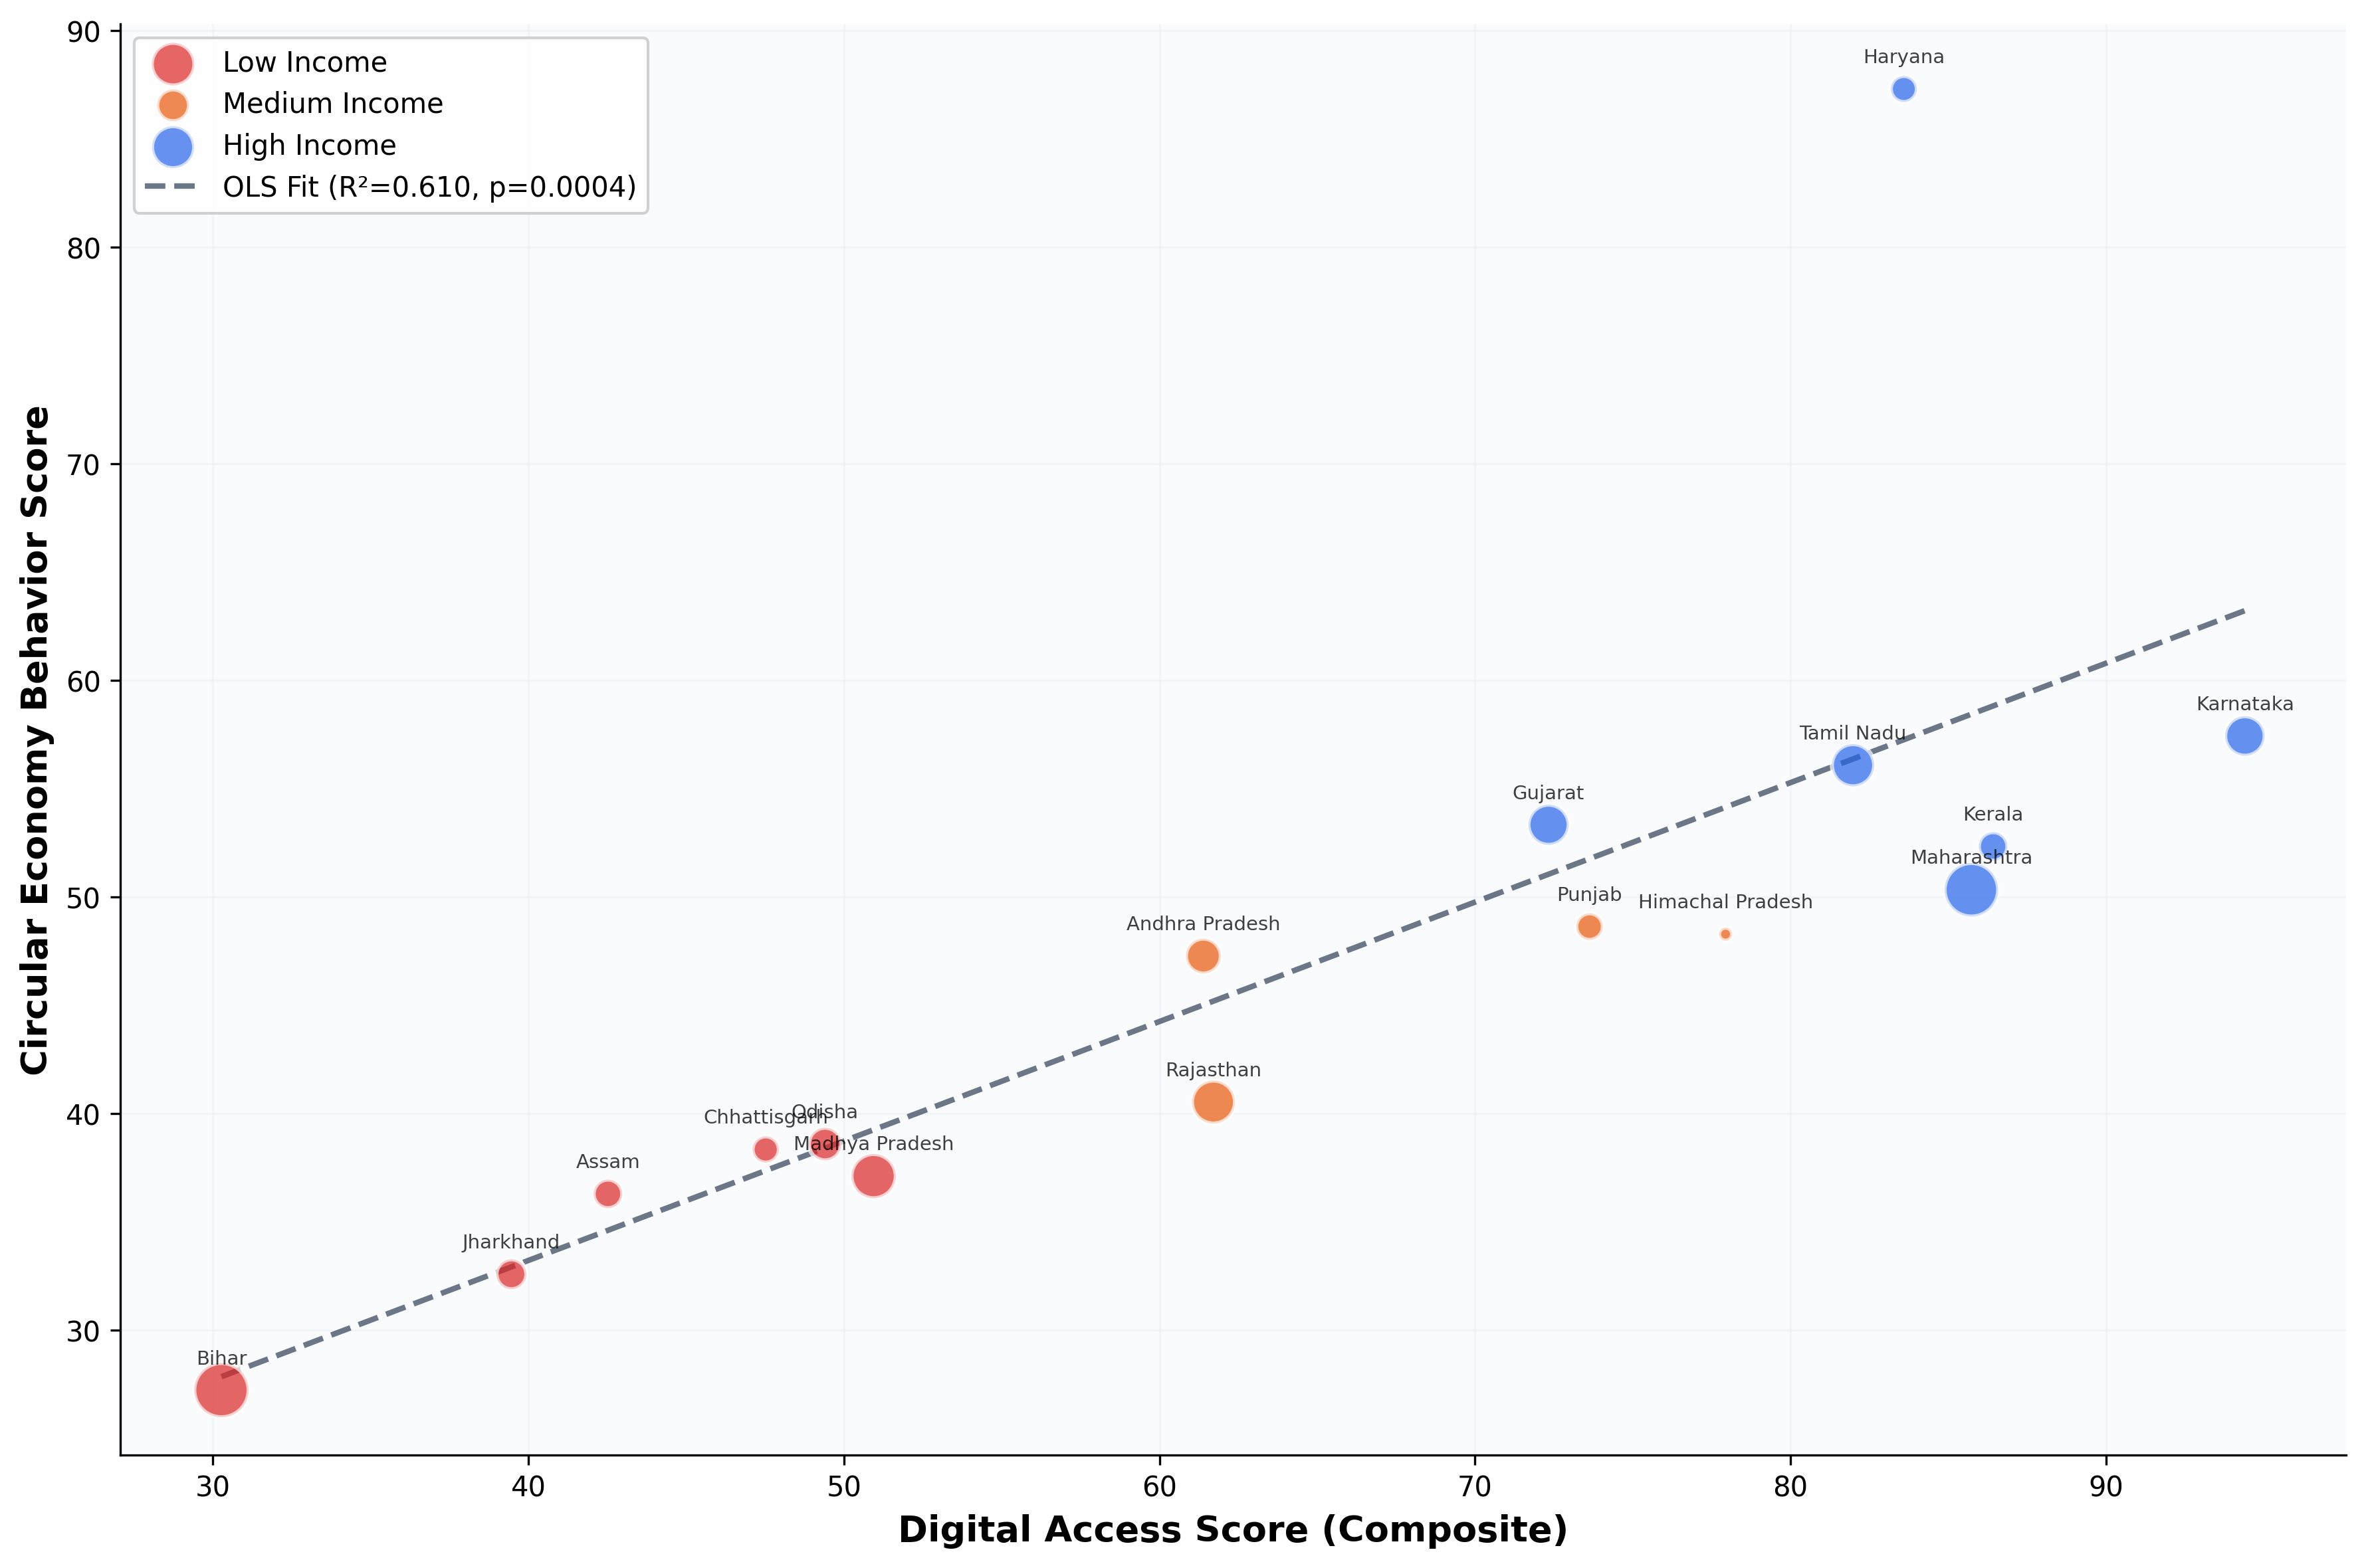
\includegraphics[width=\columnwidth]{figures/fig2_digital_vs_ce_scatter.jpg}
    \caption{Digital Access Score vs. CE Behavior Score ($r = 0.781$, $p < 0.001$). Each point represents one state.}
    \label{fig:scatter}
\end{figure}

\subsection{Robustness Checks}

Residual diagnostics showed non-normality in the OLS model and strong influence from Haryana (Cook's $D = 4.16$), so we tested the result under less favorable assumptions. Table~\ref{tab:robustness} shows that the association remains stable with HC3 standard errors, permutation testing, and rank-based statistics. It also survives alternative weighting schemes: six of seven variants produce significant Pearson correlations, and the only borderline UPI-heavy case still yields a strong Spearman correlation ($\rho = 0.882$, $p < 0.001$).

\begin{table}[!t]
\centering
\caption{Robustness Diagnostics}
\label{tab:robustness}
\renewcommand{\arraystretch}{1.15}
\begin{tabular}{@{}p{2.6cm}p{2.4cm}p{1.6cm}@{}}
\toprule
\textbf{Test} & \textbf{Value} & \textbf{Result} \\
\midrule
Spearman $\rho$        & 0.912          & $p < 0.001$ \\
Kendall $\tau$         & 0.783          & $p < 0.001$ \\
Shapiro-Wilk           & Skew = 2.72    & Non-normal \\
Breusch-Pagan LM      & 1.539          & $p = 0.215$ \\
Durbin-Watson          & 2.025          & No autocorr. \\
Cook's distance        & $D_{\max} = 4.16$ (HR) & 1 infl.\ pt. \\
Permutation $p$        & 0.0001         & Significant \\
HC3 robust $p$         & 0.000011       & Significant \\
Bootstrap CI ($r$)     & [0.648, 0.979] & Excludes 0 \\
Bootstrap CI ($\beta_1$) & [0.395, 0.836] & Excludes 0 \\
\bottomrule
\end{tabular}
\end{table}

\subsection{Mediation Analysis (H2)}

H2 tests whether UPI adoption mediates the relationship between digital access and CE behavior.

\begin{table}[!t]
\centering
\caption{Mediation Results}
\label{tab:mediation}
\renewcommand{\arraystretch}{1.15}
\begin{tabular}{@{}p{2.8cm}ccc@{}}
\toprule
\textbf{Path} & $\boldsymbol{\beta}$ & \textbf{$p$-value} & \textbf{Sig.?} \\
\midrule
$c$ (total): $X \rightarrow Y$      & 0.505 & 0.0004 & Yes \\
$a$: $X \rightarrow M$              & 1.499 & 0.003  & Yes \\
$b$: $M \rightarrow Y \mid X$       & $-$0.017 & 0.813 & No \\
$c'$ (direct): $X \rightarrow Y \mid M$ & 0.530 & 0.004 & Yes \\
Indirect ($a \times b$)             & $-$0.026 & --- & --- \\
Sobel $z$                           & $-$0.241 & 0.810 & No \\
\bottomrule
\end{tabular}
\end{table}

The evidence does not support mediation through UPI. The Sobel test is not significant ($z = -0.241$, $p = 0.810$), while the direct effect remains significant after controlling for UPI ($c' = 0.530$, $p = 0.004$). Two alternative pathways---Tele-density $\rightarrow$ NSDP $\rightarrow$ CEBS and Tele-density $\rightarrow$ SDG $\rightarrow$ CEBS---are also unsupported.

\subsection{Threshold Analysis (H3)}

The estimated tele-density breakpoint is 118.77\%:

\begin{itemize}
    \item Below that threshold, the slope is steep and positive: $\beta_1 = 0.635$ ($p = 0.0001$).
    \item Above it, the slope flips negative: $\beta_2 = -8.738$ ($p = 0.047$)---but only two or three states sit in this range, so we would not read too much into the reversal.
    \item The piecewise model fits better than the linear one: $R^2 = 0.723$ vs.\ 0.610.
\end{itemize}

These results provide qualified support for H3. CE outcomes improve sharply up to roughly 119\% tele-density, but only a few states lie above the breakpoint.

\subsection{Machine Learning Validation (LOO-CV)}

We also tested whether the signal survives out-of-sample prediction under LOO-CV.

\begin{table}[!t]
\centering
\caption{ML Model Comparison --- LOO-CV Results}
\label{tab:ml_loocv}
\renewcommand{\arraystretch}{1.15}
\begin{tabular}{@{}p{1.8cm}cccc@{}}
\toprule
\textbf{Model} & \multicolumn{2}{c}{\textbf{Digital-Only}} & \multicolumn{2}{c}{\textbf{Full Model}} \\
\cmidrule(lr){2-3} \cmidrule(lr){4-5}
 & $R^2$ & $r$ & $R^2$ & $r$ \\
\midrule
ElasticNet & \textbf{0.364} & 0.603 & 0.534 & 0.731 \\
Lasso      & 0.347 & 0.606 & \textbf{0.568} & 0.758 \\
Ridge      & 0.338 & 0.597 & 0.536 & 0.743 \\
RF         & 0.326 & 0.575 & 0.490 & 0.703 \\
Lin. Reg.  & 0.301 & 0.585 & 0.442 & 0.713 \\
SVR (RBF)  & 0.286 & 0.554 & 0.425 & 0.700 \\
GB         & 0.161 & 0.542 & 0.445 & 0.687 \\
\bottomrule
\end{tabular}
\end{table}

Even with only the three digital-access variables, ElasticNet explains 36\% of the out-of-sample variance in CE behavior ($p = 0.013$). The best full-model LOO-CV result (Lasso, $R^2 = 0.568$) also remains close to the OLS value of 0.610.

\subsection{Nested LOO-CV (Leak-Free Evaluation)}

To remove hyperparameter optimism from standard LOO-CV, we used a nested design with an outer LOO loop and an inner 4-fold tuning loop.

\begin{table}[!t]
\centering
\caption{Nested LOO-CV Results (Leak-Free)}
\label{tab:nested_cv}
\renewcommand{\arraystretch}{1.15}
\begin{tabular}{@{}lccc@{}}
\toprule
\textbf{Model} & \textbf{Nested $R^2$} & \textbf{RMSE} & \textbf{$r$} \\
\midrule
\textbf{XGBoost} & \textbf{0.511} & 9.41 & 0.721 \\
Random Forest    & 0.504          & 9.48 & 0.711 \\
ElasticNet       & 0.471          & 9.78 & 0.723 \\
Ridge            & 0.445          & 10.03 & 0.714 \\
Lasso            & 0.443          & 10.05 & 0.713 \\
SVR              & $-$0.023       & 13.61 & $-$0.593 \\
\bottomrule
\end{tabular}
\end{table}

XGBoost performs best under this stricter setup, reaching $R^2 = 0.511$ ($p = 0.002$), while SVR falls below a mean-prediction baseline. In repeated 4-fold CV, Random Forest shows the tightest distribution, with Mean $R^2 = 0.442$ and Median $R^2 = 0.603$.

\subsection{SHAP Explainability Analysis}

SHAP values were computed for all six features across all 16 states.

\begin{table}[!t]
\centering
\caption{SHAP Global Feature Importance}
\label{tab:shap}
\renewcommand{\arraystretch}{1.15}
\begin{tabular}{@{}clc@{}}
\toprule
\textbf{Rank} & \textbf{Feature} & \textbf{Mean $|\phi|$} \\
\midrule
1 & Tele-density (\%)          & \textbf{5.012} \\
2 & Per Capita NSDP            & 4.883 \\
3 & Population (Mn)            & 1.714 \\
4 & Urban (\%)                 & 1.677 \\
5 & Literacy Rate (\%)         & 0.998 \\
6 & UPI Per Capita             & 0.914 \\
\bottomrule
\end{tabular}
\end{table}

Tele-density ranks first (mean $|\phi| = 5.01$), with Per Capita NSDP close behind at 4.88. UPI ranks last at 0.91. Figs.~\ref{fig:shap_beeswarm} and \ref{fig:shap_waterfall} show the same pattern at both global and state levels.

\begin{figure}[!t]
    \centering
    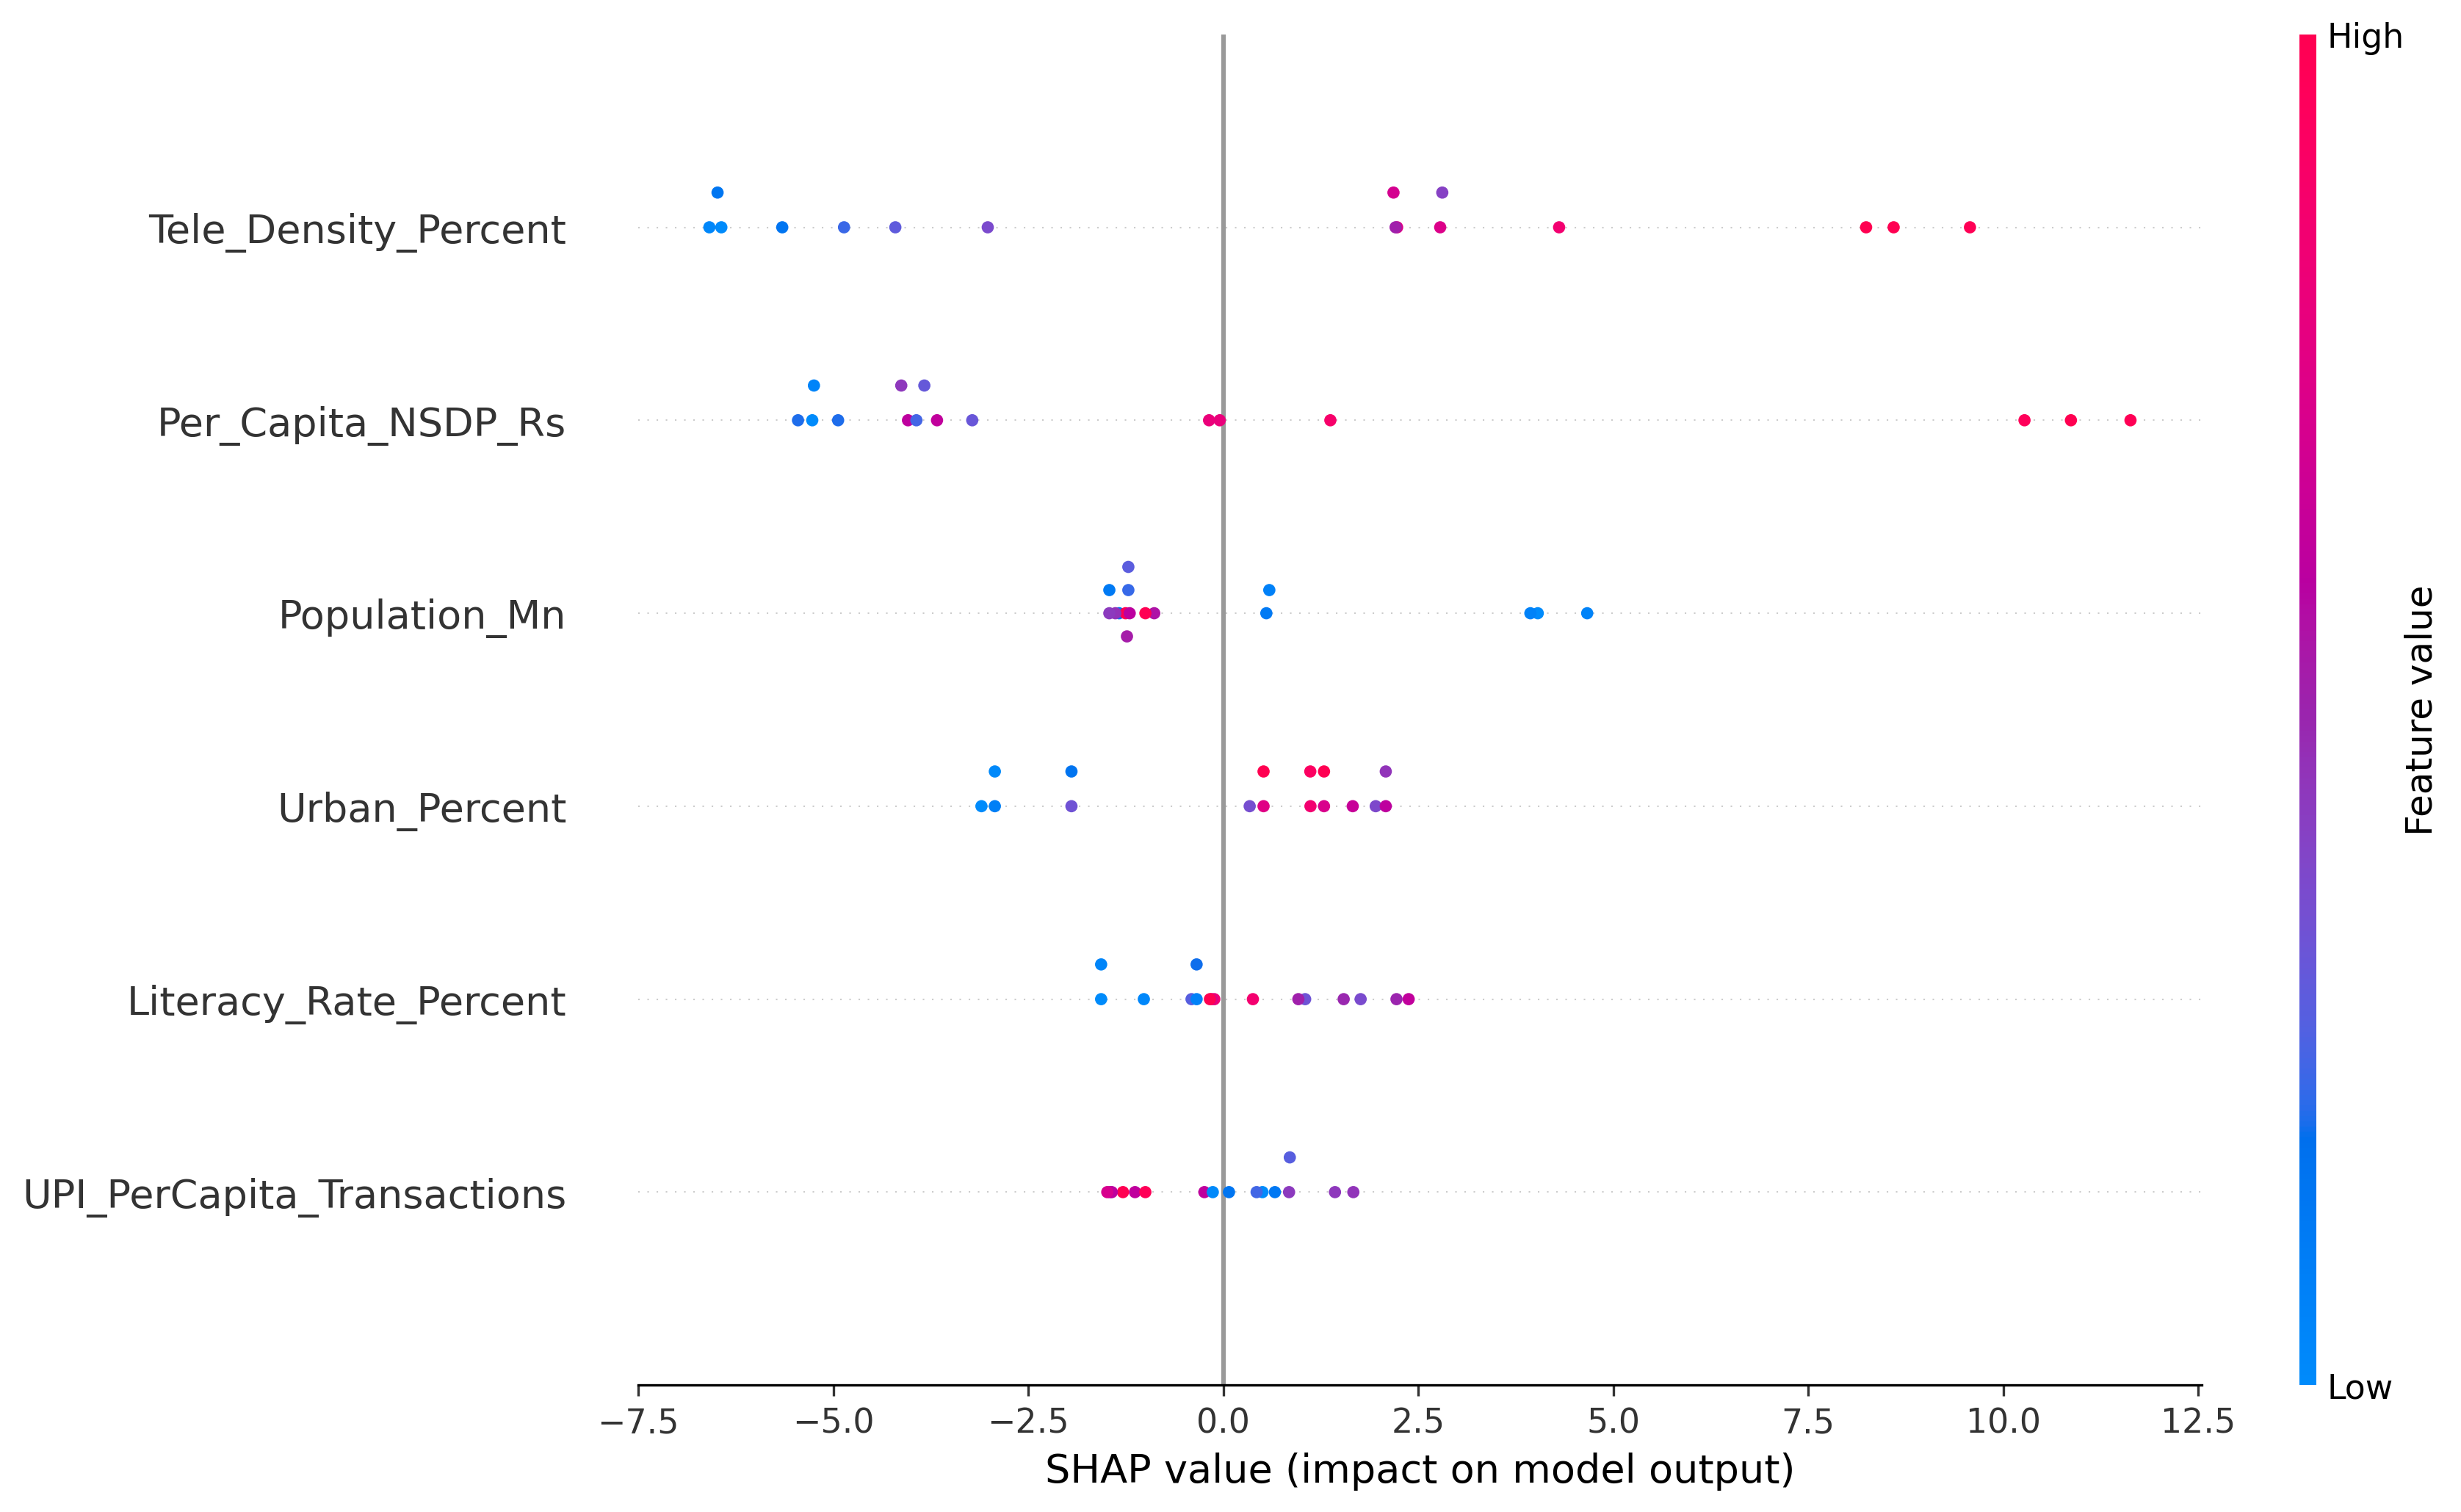
\includegraphics[width=\columnwidth]{figures/fig17_shap_beeswarm.jpg}
    \caption{SHAP beeswarm plot. Each dot represents one state for one feature. Color indicates feature value (red = high, blue = low). Tele-density and NSDP have the widest spread.}
    \label{fig:shap_beeswarm}
\end{figure}

\begin{figure}[!t]
    \centering
    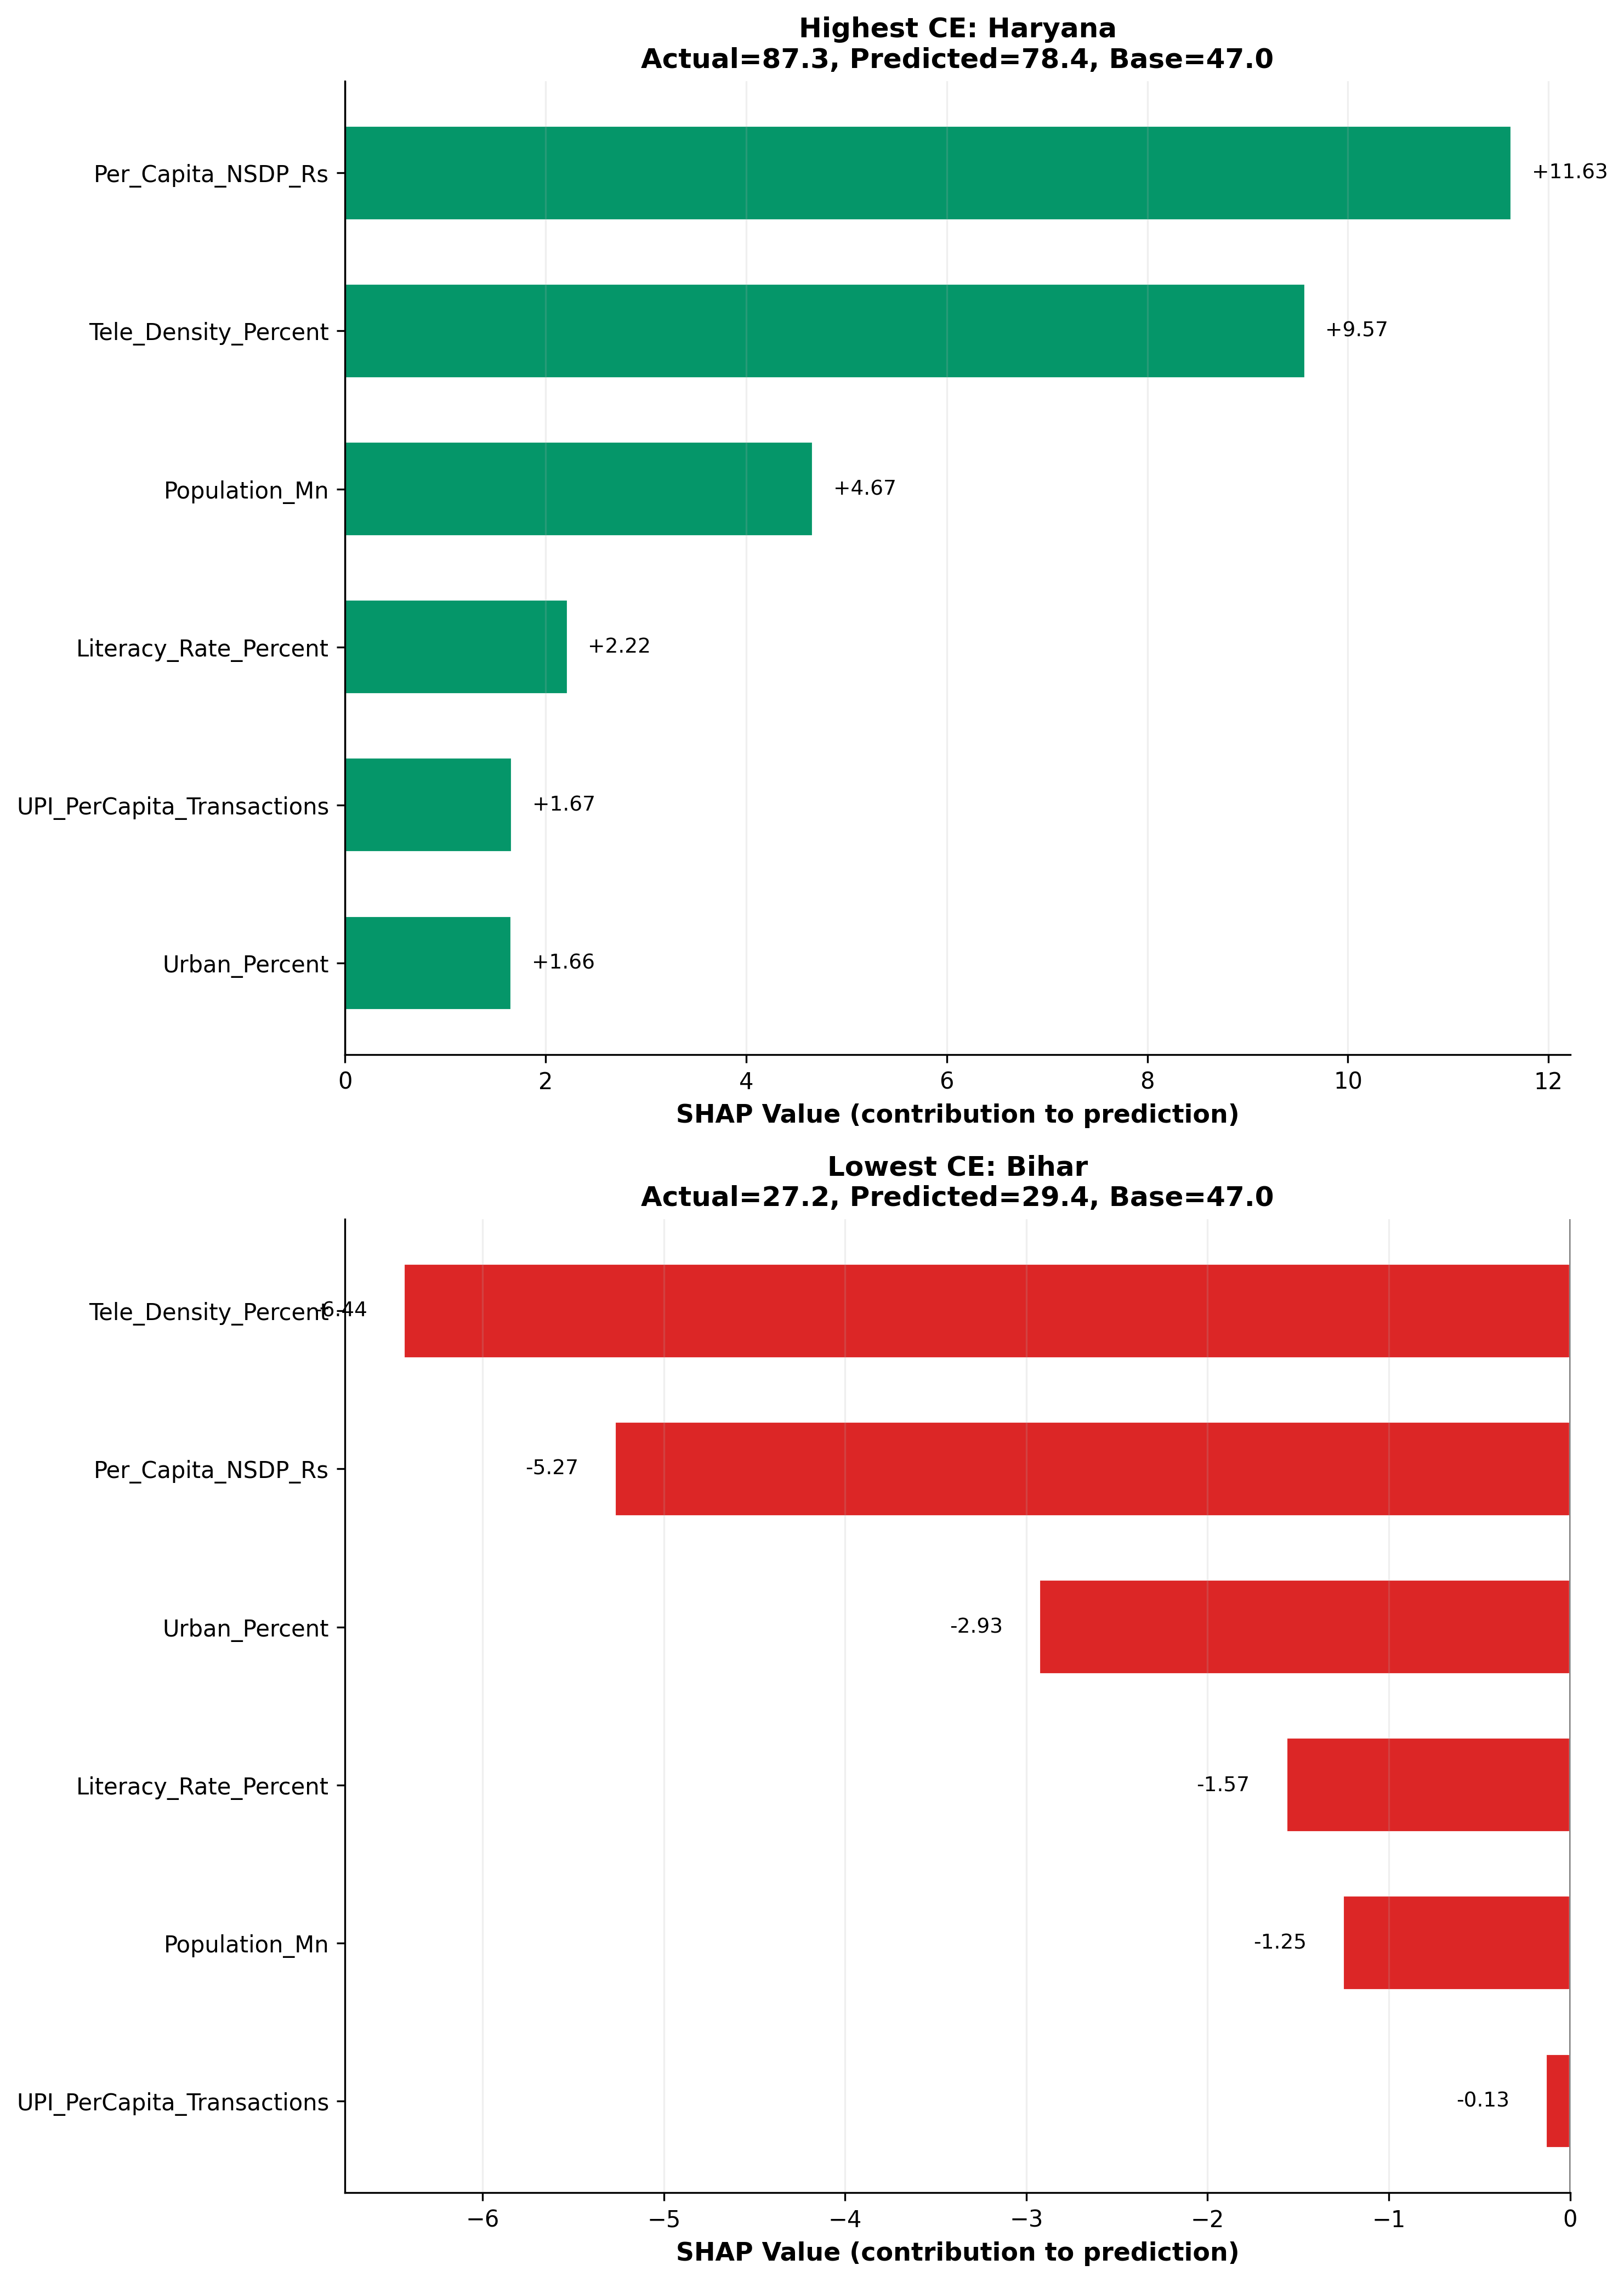
\includegraphics[width=\columnwidth]{figures/fig19_shap_waterfall.jpg}
    \caption{SHAP waterfall explanations. Left: Haryana (highest CE)---high NSDP (+11.63) and tele-density (+9.57) push score up. Right: Bihar (lowest CE)---low tele-density ($-$6.44) and NSDP ($-$5.27) push score down.}
    \label{fig:shap_waterfall}
\end{figure}

\subsection{K-Means Clustering (State Typologies)}

K-Means clustering produced a best-fit solution of $k = 2$ (Table~\ref{tab:clusters}). The two groups correspond to \textbf{Digital Leaders} and \textbf{Emerging States}.

\begin{table}[!t]
\centering
\caption{K-Means Cluster Profiles}
\label{tab:clusters}
\renewcommand{\arraystretch}{1.15}
\begin{tabular}{@{}p{2.1cm}cccl@{}}
\toprule
\textbf{Cluster} & \textbf{$n$} & \textbf{DAS} & \textbf{CEBS} & \textbf{DCI} \\
\midrule
Digital Leaders  & 8 & 82.0 & 56.7 & \textbf{46.7} \\
Emerging\newline States  & 8 & 47.9 & 37.2 & 18.3 \\
\midrule
\textbf{Gap}     & --- & 34.1 & 19.5 & \textbf{28.4} \\
\bottomrule
\end{tabular}
\end{table}

The separation is substantial: average DCI differs by roughly 2.5$\times$ (46.7 vs.\ 18.3). PCA reinforces the same interpretation, with the first component explaining 62.3\% of the variance.

\subsection{Extended Sample Validation}

As an extended-sample check, we removed e-waste from CEBS and recalculated the analysis, increasing the sample to $n = 21$. The relationship became stronger rather than weaker: Pearson $r = 0.963$ ($p < 0.000001$), Spearman $\rho = 0.951$, and OLS $R^2 = 0.927$.

\begin{figure}[!t]
    \centering
    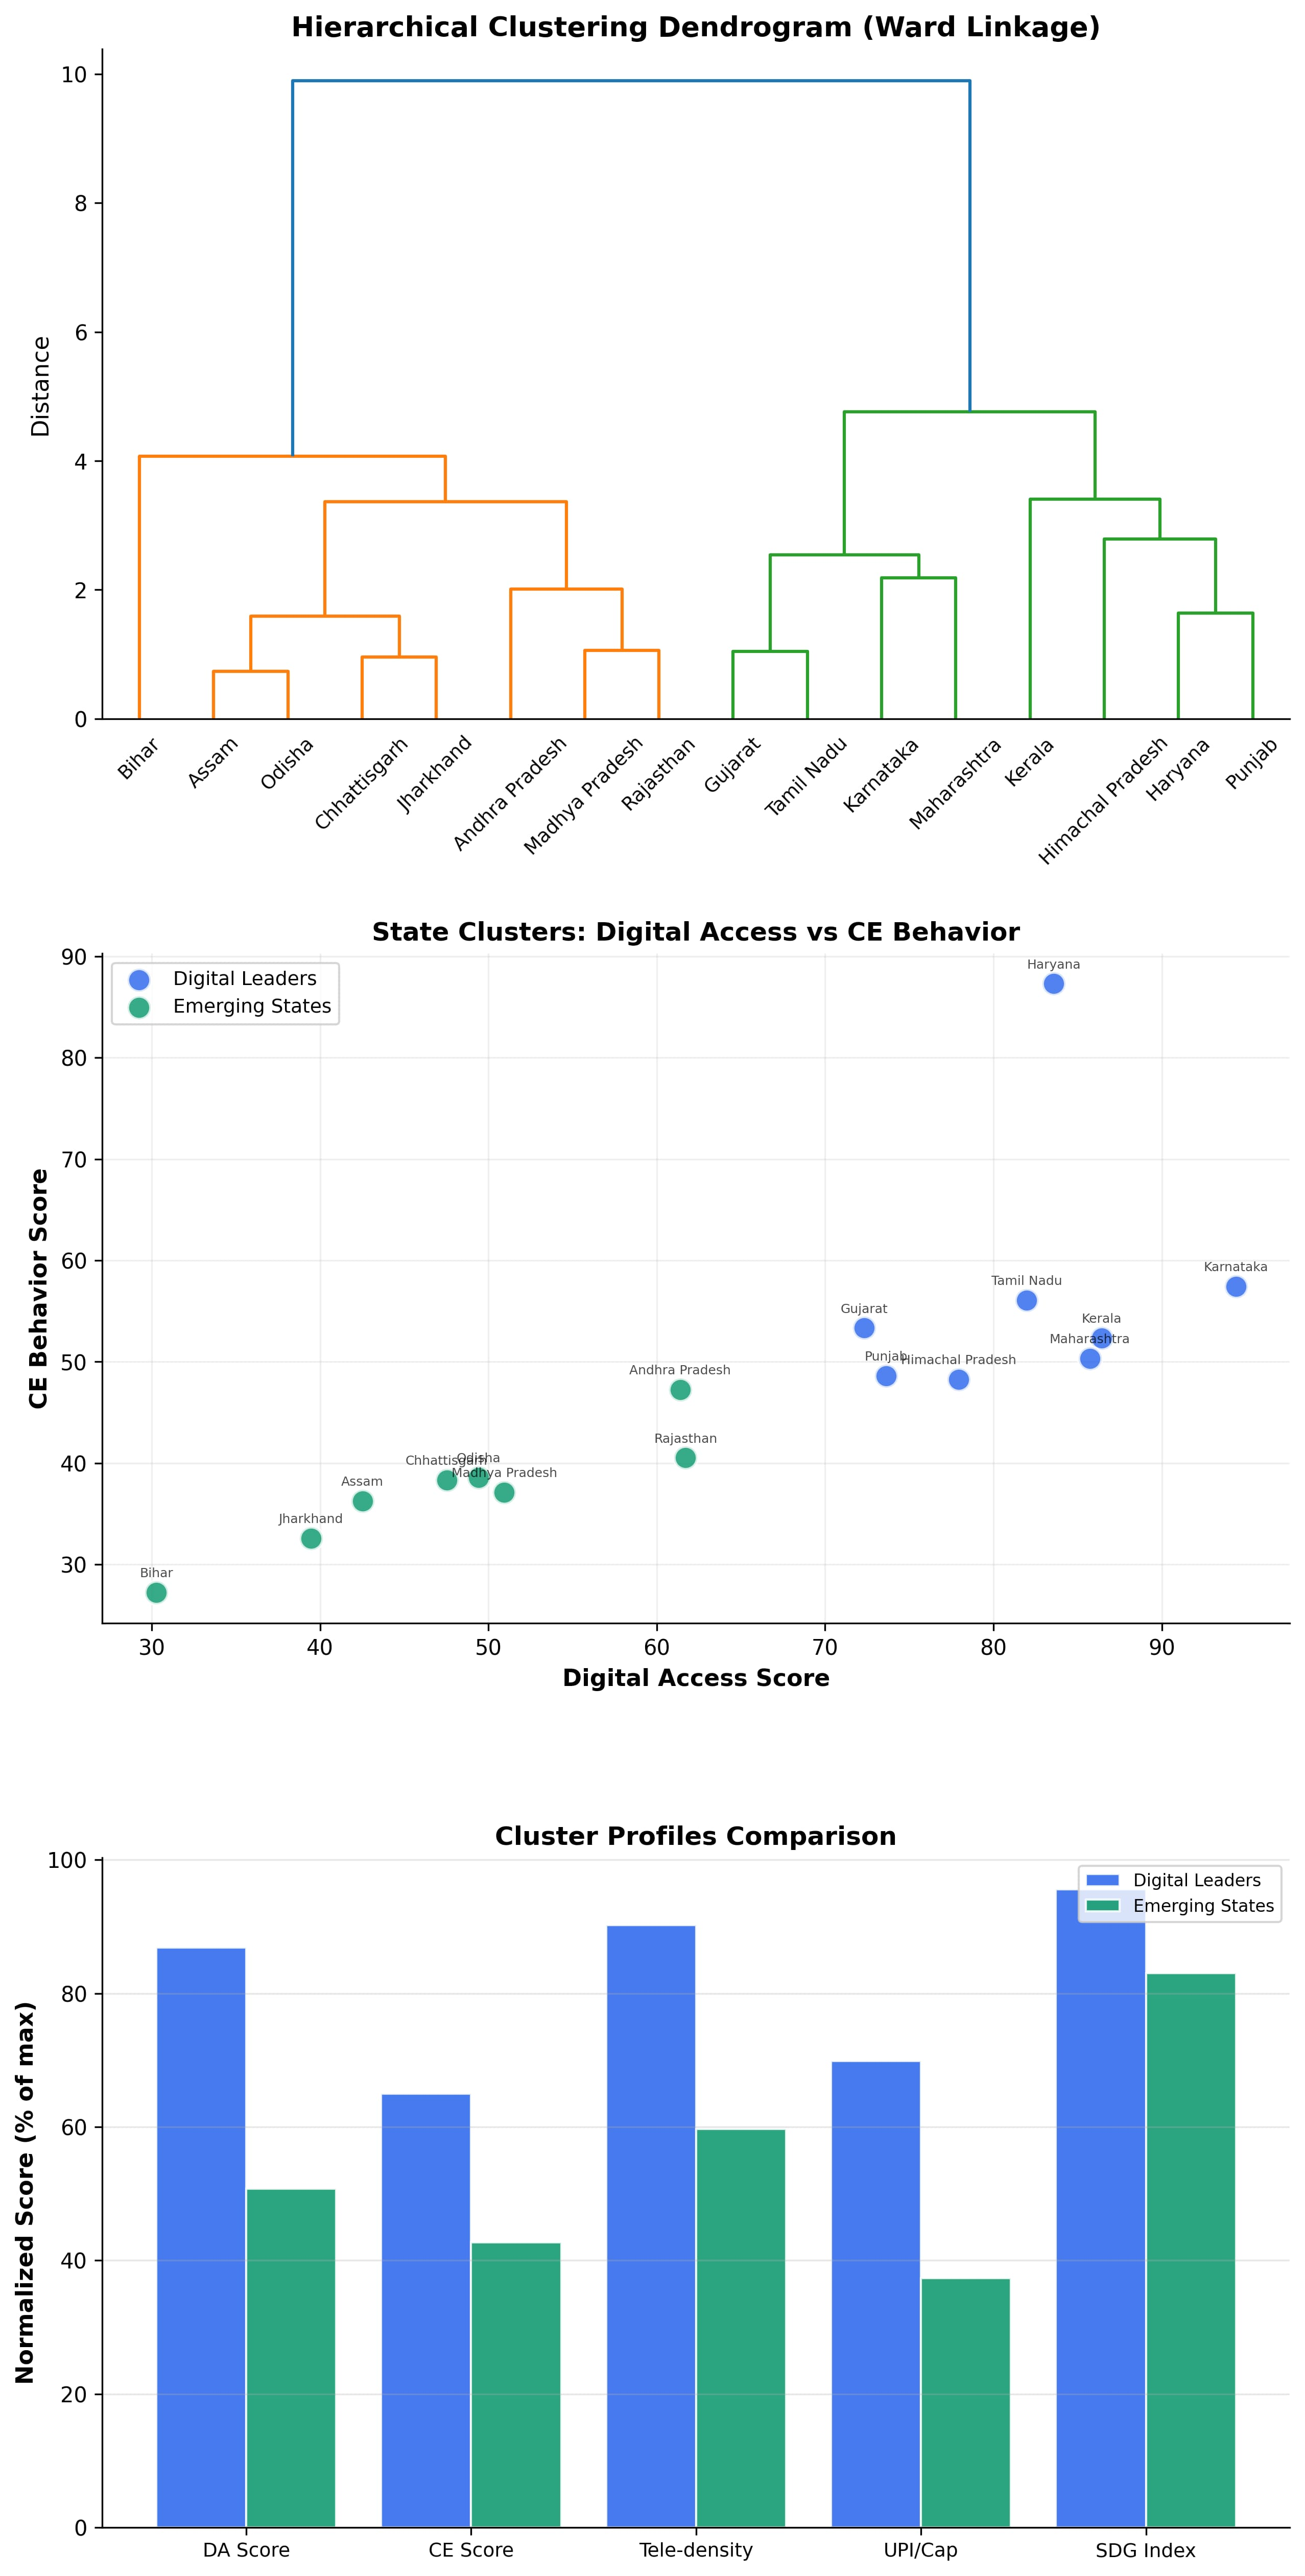
\includegraphics[width=\columnwidth]{figures/fig20_clustering.jpg}
    \caption{K-Means clustering results with hierarchical dendrogram and cluster radar profiles. Two distinct state typologies emerge.}
    \label{fig:clustering}
\end{figure}

% ============================================================================
% V. DISCUSSION
% ============================================================================
\section{Discussion}

\subsection{Do the Methods Agree?}

Broadly, yes. The OLS model explains 61\% of the variance, while nested-CV XGBoost explains 51.1\%. The expected drop from in-sample to out-of-sample performance does not change the main point: the relationship remains positive and significant across parametric, non-parametric, and predictive methods. For a 16-state sample, that consistency is meaningful evidence against a simple overfitting story.

\subsection{What Drives the Relationship?}

The feature-importance results differ in emphasis but not in substance: Random Forest favors Per Capita NSDP, while SHAP favors tele-density. Both methods nonetheless identify tele-density and NSDP as the two main drivers. UPI is the more unexpected result. It receives the smallest SHAP contribution, and the Sobel test is not significant ($z = -0.241$, $p = 0.810$), suggesting that digital access matters less through payments alone than through broader infrastructure and institutional capacity \cite{avgerou2010,heeks2017}.

\subsection{The Two Indias in CE Performance}

The clustering results sharpen the divide: one group is strong on both digital access and CE outcomes, while the other is weak on both. The DCI gap---46.7 versus 18.3---suggests not a mild gradient but two distinct development settings, with the digital divide carrying a clear sustainability dimension.

\subsection{What This Means for Policy}

\begin{enumerate}
    \item Digital India and Swachh Bharat should be treated less as separate policy tracks and more as connected systems.
    \item Connectivity investment in lagging states should be viewed not only as a telecom intervention but also as part of environmental capacity-building.
    \item Because UPI is not the mediating channel, digital inclusion policy should extend beyond payments to reporting systems, e-governance, and digital literacy.
    \item The two clusters argue against a single national playbook: Digital Leaders can move toward advanced monitoring, while Emerging States need basic infrastructure first.
    \item SHAP highlights state-specific constraints, suggesting that uniform intervention design would miss important differences.
\end{enumerate}

\subsection{Limitations and Future Work}

The study has clear limits. The final sample contains only 16 states because we retain only complete and directly comparable observations across all seven sources. That improves traceability but increases sensitivity to influential cases such as Haryana (Cook's $D = 4.16$). The bootstrap intervals and 21-state validation strengthen confidence in the result, but they do not remove the small-sample constraint.

The design is also cross-sectional, so the analysis supports association rather than causation. Stronger causal claims would require panel data and designs that can separate policy effects from background factors such as governance quality and long-run development differences.

Measurement constraints remain. Literacy and urbanisation still come from the 2011 Census, NSDP enters both DAS and CEBS, and state averages compress large within-state variation. Future work should therefore use district-level or panel data, expand the CE index with measures such as plastic recovery and EPR compliance, and test the framework in other countries with comparable administrative data.

% ============================================================================
% VI. CONCLUSION
% ============================================================================
\section{Conclusion}

This study finds a consistent state-level association between digital access and circular-economy behavior in India. Across the 16 states retained in the final dataset, the pattern remains visible under both statistical and machine-learning approaches: the OLS model gives $r = 0.781$ ($p < 0.001$), while leak-free nested-CV XGBoost still reaches $R^2 = 0.511$.

Tele-density matters more than digital payments in explaining the observed pattern, and the clustering analysis reinforces the same message by separating states into two groups with a 2.5$\times$ DCI gap. Taken together, these results suggest that digital inclusion and circular-economy policy should be treated as connected rather than separate agendas.

% ============================================================================
% ACKNOWLEDGMENT
% ============================================================================
\section*{Acknowledgment}

The authors acknowledge the Telecom Regulatory Authority of India, the Reserve Bank of India, NITI Aayog, the National Payments Corporation of India, and the Central Pollution Control Board for maintaining the public datasets used in this study.

% ============================================================================
% REFERENCES
% ============================================================================
\balance
\begin{thebibliography}{00}

\bibitem{npci2025}
NPCI, ``UPI Product Statistics (Monthly),'' National Payments Corporation of India, Mumbai, 2025. [Online]. Available: \url{https://www.npci.org.in/what-we-do/upi/product-statistics}

\bibitem{trai2024}
TRAI, ``Indian Telecom Services Performance Indicators Report: April--June 2024,'' Telecom Regulatory Authority of India, New Delhi, 2024. [Online]. Available: \url{https://www.trai.gov.in/sites/default/files/2024-09/IndicatorReport1oct09.pdf}

\bibitem{cpcb2023}
CPCB, ``Annual Report on Implementation of E-Waste (Management) Rules, 2016 for FY 2021--22,'' Central Pollution Control Board, Ministry of Environment, Forest and Climate Change, Government of India, 2023. [Online]. Available: \url{https://cpcb.nic.in/e-waste/}

\bibitem{nitiCE2021}
NITI Aayog, ``Circular Economy in India: Rethinking Growth for Long-Term Prosperity,'' Government of India, New Delhi, 2021.

\bibitem{meity2023}
Ministry of Electronics \& IT, ``Digital India Programme: Progress and Initiatives,'' Government of India, 2023. [Online]. Available: \url{https://digitalindia.gov.in}

\bibitem{geissdoerfer2017}
M. Geissdoerfer, P. Savaget, N. M. Bocken, and E. J. Hultink, ``The Circular Economy -- A new sustainability paradigm?'' \textit{J. Cleaner Prod.}, vol. 143, pp. 757--768, 2017.

\bibitem{emf2013}
Ellen MacArthur Foundation, ``Towards the Circular Economy: Economic and Business Rationale for an Accelerated Transition,'' 2013. [Online]. Available: \url{https://ellenmacarthurfoundation.org}

\bibitem{nitiSDG2024}
NITI Aayog, ``SDG India Index \& Dashboard 2023--24,'' 4th ed., National Institution for Transforming India, Government of India, New Delhi, 2024. [Online]. Available: \url{https://sdgindiaindex.niti.gov.in}

\bibitem{avgerou2010}
C. Avgerou, ``Discourses on ICT and development,'' \textit{Inf. Technol. Int. Dev.}, vol. 6, no. 3, pp. 1--18, 2010.

\bibitem{heeks2017}
R. Heeks, \textit{Information and Communication Technology for Development (ICT4D)}. Routledge, 2017.

\bibitem{rbi2025}
RBI, ``Handbook of Statistics on Indian Economy 2024--25, Table 9: Per Capita Net State Domestic Product,'' Reserve Bank of India, Mumbai, 2025. [Online]. Available: \url{https://www.rbi.org.in/scripts/AnnualPublications.aspx?head=Handbook+of+Statistics+on+Indian+Economy&lang=en}

\bibitem{dataful2026}
Dataful Insights, ``Here is How UPI Usage Differs Across Indian States,'' Factly Media \& Research, Jan. 23, 2026. [Online]. Available: \url{https://insights.dataful.in/articles/here-is-how-upi-usage-differs-across-indian-states}

\bibitem{census2011}
Census of India, ``Primary Census Abstract: Literacy Rate, Level of Urbanization, Population,'' Office of the Registrar General \& Census Commissioner, Ministry of Home Affairs, Government of India, 2011. [Online]. Available: \url{https://censusindia.gov.in}

\bibitem{baron1986}
R. M. Baron and D. A. Kenny, ``The moderator-mediator variable distinction in social psychological research: Conceptual, strategic, and statistical considerations,'' \textit{J. Pers. Soc. Psychol.}, vol. 51, no. 6, pp. 1173--1182, 1986.

\bibitem{lundberg2017}
S. M. Lundberg and S.-I. Lee, ``A Unified Approach to Interpreting Model Predictions,'' in \textit{Advances in Neural Information Processing Systems (NeurIPS)}, vol. 30, 2017.

\end{thebibliography}

\end{document}
